\documentclass{beamer}

%\usepackage{siunitx} 
\usepackage{multicol} 
\usepackage{listings}

\usetheme{Rochester} 
\usecolortheme{material}

\setbeamertemplate{footline}[text line]{

%
\parbox{0.5\linewidth}{ \vspace*{-12pt} 

%\insertshorttitle~(\insertshortauthor)
} \hfill

%
\parbox{0.5\linewidth}{ \vspace*{-12pt} 
\raggedleft\insertpagenumber } } \lstset{ breaklines=true, basicstyle=\scriptsize, keywordstyle=\color{blue700}, basewidth=0.55em } \setbeamertemplate{navigation symbols}{} \begin{document} 
\title[Massively Parallelized Iris Recognition with CUDA]{Massively Parallelized Iris Recognition with CUDA} 
\author[Platzer M., Weber T., Zaruba F.]{Platzer Michael, Weber Thomas, Zaruba Florian} 
\date{\today} 
\begin{frame}
	\titlepage 
\end{frame}

% \begin{frame}\frametitle{Table of Contents}
% \begin{multicols}{2}
%   \tableofcontents
% \end{multicols}
% \end{frame}
\section{Introduction} 
\subsection{Iris Recognition} 
\begin{frame}\frametitle{Motivation} 
	\begin{itemize}
		\item Iris recognition is one of the most accurate biometric methods.
		\item Computationally intensive but highly parallelizable.
		\item Iris recognition on GPU (with CUDA) is a novel approach (only FPGA and parallel CPU implementations have been done before).
		\item Has industry relevant use cases (e.g.: Windows Hello \footnote{\url{https://blogs.windows.com/bloggingwindows/2015/03/17/making-windows-10-more-personal-and-more-secure-with-windows-hello/}}, sophisticated surveillance systems)
		\item Can the iris be recognized in real-time using CUDA (or even the Tegra architecture)?
	\end{itemize}
\end{frame}

\subsection{System Overview} 
\begin{frame}
	\frametitle{System Overview} 
	\begin{figure}
		[ht] \centering 
		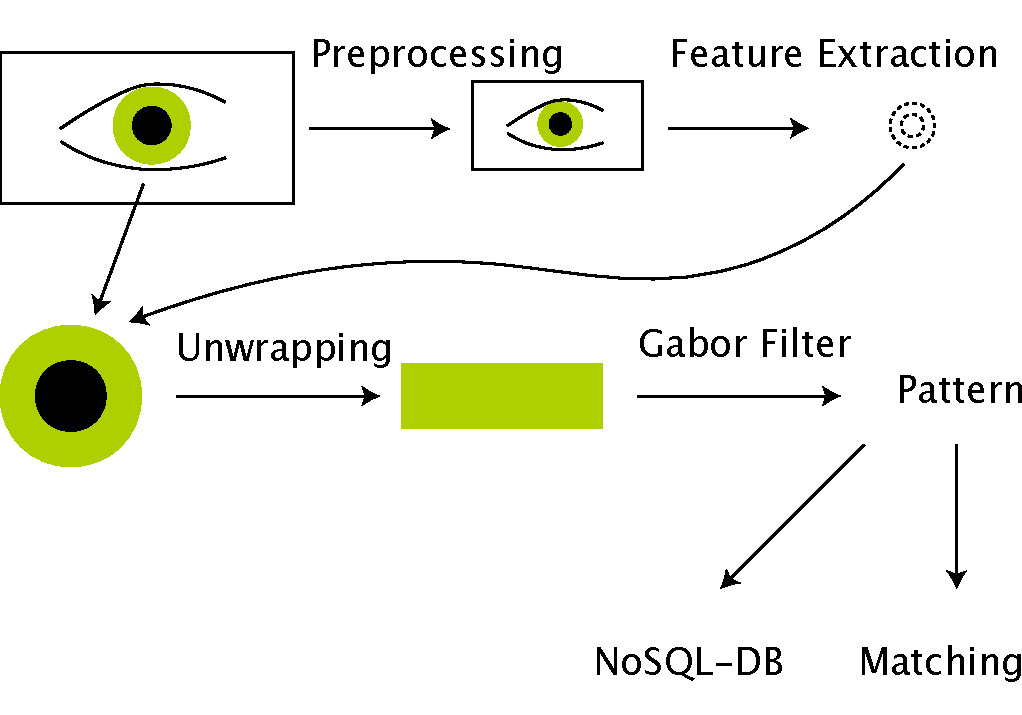
\includegraphics[width=0.85
		\textwidth]{../report/iris/flow} \caption{Program flow of iris detection} \label{fig:flow} 
	\end{figure}
\end{frame}
\section{Approach} 
\subsection{Preprocessing} 
\begin{frame}
	[fragile] \frametitle{Preprocessing - Resizeing and Bluring} 
	\begin{columns}
		\begin{column}
			{0.5
			\textwidth} 
			\begin{itemize}
				\item Reduces the amount of data necessary to handle upcoming tasks. 
				\item Noise reduction 
			\end{itemize}
		\end{column}
		\begin{column}
			{0.5
			\textwidth} 
			\begin{figure}
				[ht] \centering 
				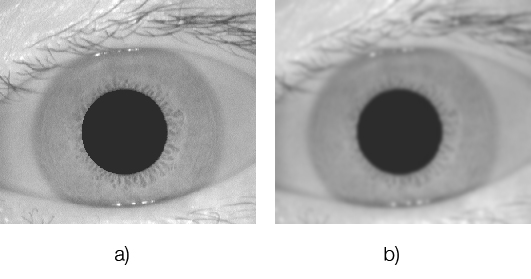
\includegraphics[width=0.99
				\textwidth]{../report/iris/resized.jpg} \caption{a) Test image from the CASIA Iris Image Database for Testing Version 1.0~\cite{ir-testv1}. b) Image after Gaussian blur.} \label{fig:input} 
			\end{figure}
		\end{column}
	\end{columns}
\end{frame}
\begin{frame}
	[fragile] \frametitle{Improvement - Seperable Convolution} Example of a separable convolution matrix (Sobel operation): $$
	\begin{bmatrix}
		-1&0&1\\-2&0&2\\-1&0&1
	\end{bmatrix}
	=
	\begin{bmatrix}
		1\\2\\1
	\end{bmatrix}
	\begin{bmatrix}
		-1&0&1
	\end{bmatrix}
	$$ 
	\begin{itemize}
		\item Instead of $n*m$ multiplications for each output pixel, where $n$ and $m$ are the width and height of the image only $n+m$ multiplications are needed. 
		\item Loop unrolling and compile time optimizations. 
	\end{itemize}
\end{frame}

\subsection{Feature Extraction} 
\begin{frame}
	[fragile] \frametitle{Center detection} 
	\begin{columns}
		\begin{column}
			{0.5
			\textwidth} 
			\begin{enumerate}
				[1.] 
				\item Edge detection with Sobel operation (see previous slide) 
				\item Hough operation - feature extraction technique mostly concerned with finding imperfect instances of certain parameterized curves \cite{shapiro2001computer}. 
				\begin{itemize}
					\item Iterates through all possible $(x,y)$-coordinates. 
					\item For each pixel look for perpendicular lines. 
					\item Increment a local accumulator. 
				\end{itemize}
			\end{enumerate}
		\end{column}
		\begin{column}
			{0.5
			\textwidth} 
			\begin{figure}
				[ht] \centering 
				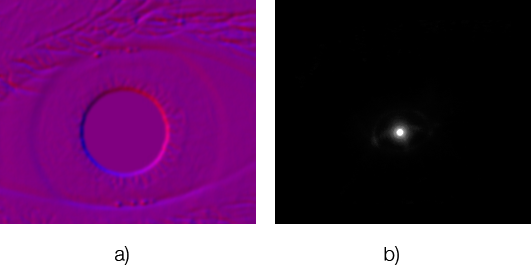
\includegraphics[width=0.99
				\textwidth]{../report/iris/sobel_hough.png} \caption{a) Gradient map after Sobel opration (blue gradient component in x-direction and red gradient component in y-direction) b) heat map of center detection; center of gravity at (123, 133) pixels (at an overall image size of 320 pixels width and 280 pixels height).} \label{fig:sobel_hough} 
			\end{figure}
		\end{column}
	\end{columns}
\end{frame}
\begin{frame}
	[fragile] \frametitle{Hough Transform - CUDA improvements} 
	\begin{columns}
		\begin{column}
			{0.5
			\textwidth} 
			\begin{itemize}
				\item Texture memory: Algorithm has high spatial locality - no boundary checks. 
				\item Loop unrolling 
				\item Reduction algorithm: Using atomic and warp functions. 
			\end{itemize}
		\end{column}
		\begin{column}
			{0.5
			\textwidth} 
			\begin{figure}
				[ht] \centering 
				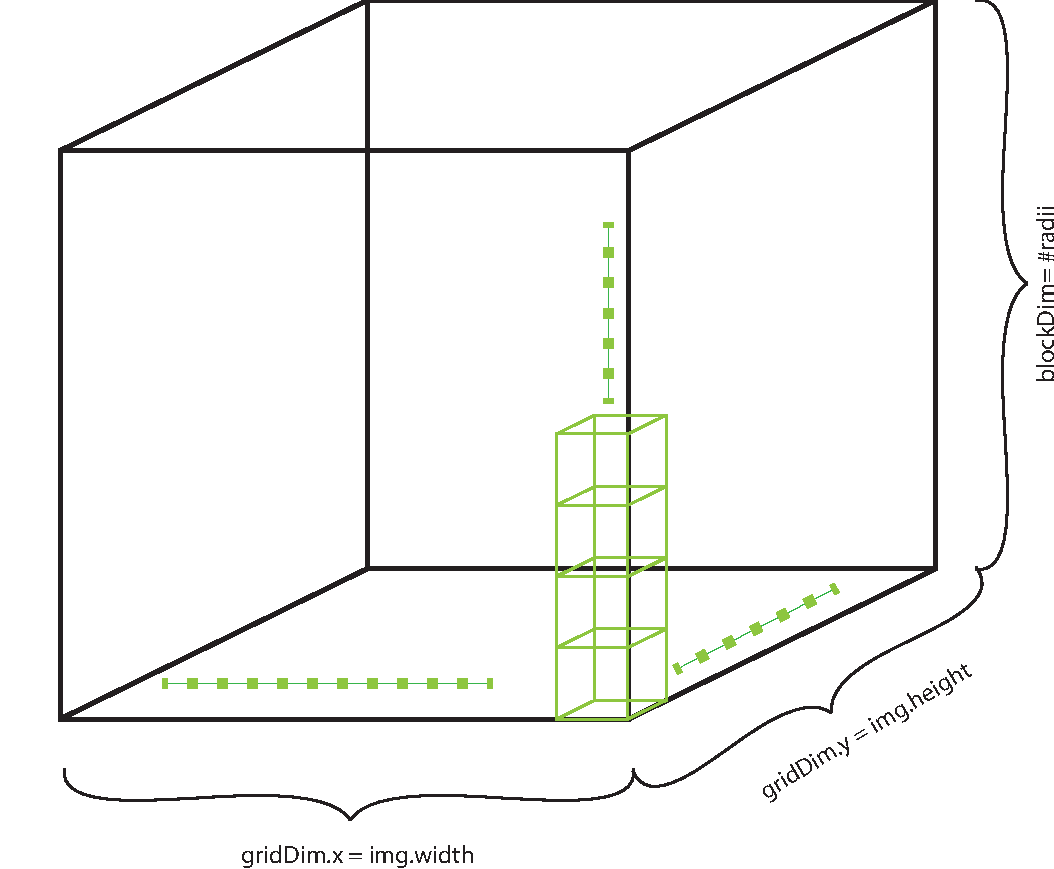
\includegraphics[width=0.999
				\textwidth]{../report/iris/hough_impl} \caption{Thread structure of Hough transformation} \label{fig:hough_impl} 
			\end{figure}
		\end{column}
	\end{columns}
\end{frame}
\begin{frame}
	[fragile] \frametitle{Radii detection} 
	\begin{columns}
		\begin{column}
			{0.5
			\textwidth} 
			\begin{itemize}
				\item Favor pixels that are circular to the detected center. Multiplication with a Gaussian circular to the center. 
				\item Unroll image regarding to the center (figure a). 
				\item Search for local maxima (figure b). 
				\item Decide for contour lines. Bayesian decision approach (figure c). 
			\end{itemize}
		\end{column}
		\begin{column}
			{0.5
			\textwidth} 
			\begin{figure}
				[ht] \centering 
				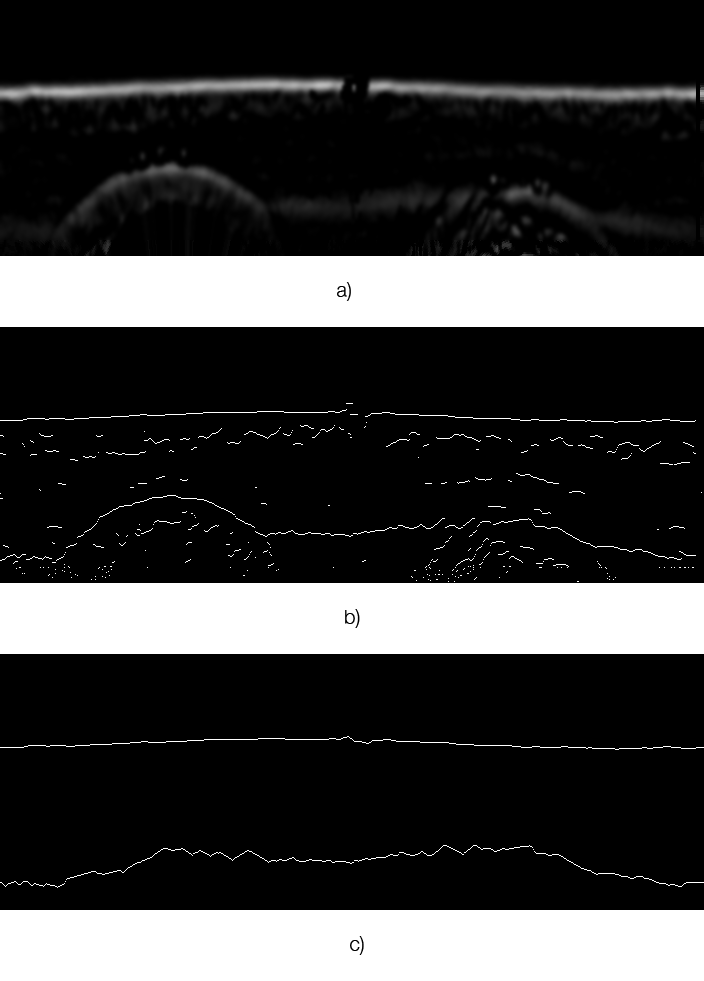
\includegraphics[width=0.89
				\textwidth]{../report/iris/unrolled.png} \label{fig:hough_impl} 
			\end{figure}
		\end{column}
	\end{columns}
\end{frame}
\begin{frame}
	[fragile] \frametitle{Contour line tracing} 
	\begin{itemize}
		\item Traverse image from left to right. 
		\item 60 pixel look ahead. 
		\item Assert different costs to different traces $\rightarrow$ pick the two traces with the lowest costs. 
	\end{itemize}
	\begin{figure}
		[ht] \centering 
		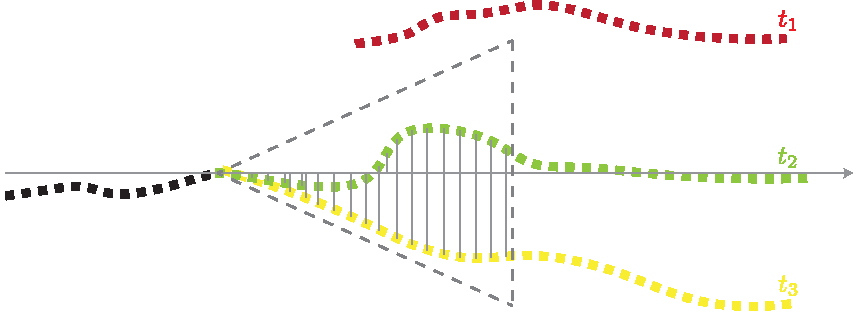
\includegraphics[width=0.79
		\textwidth]{../report/iris/trace} \caption{The tracing process is depicted for 3 different traces $t_1$, $t_2$ and $t_3$. While $t_1$ is not recognized $t_2$ has a lower cost function assigned than $t_3$.} \label{fig:trace} 
	\end{figure}
\end{frame}
\subsection{Unrolling} 
\begin{frame}
	[fragile] \frametitle{Unrolling} 
	\begin{columns}
		\begin{column}
			{0.5
			\textwidth} 
			\begin{itemize}
				\item Unrolling with regard to the trace determined in the previous step. 
				\item In order to enhance the performance in the later step of pattern matching we are equalizing the image over the whole grey space of 256 bit. 
				\item 
%				\begin{aligned}
%					& cdf_x(i) = \sum \limits_{j=0}^{i} p_x(j) \\
%					& pal(i) = cdf_x(i)\cdot 255 
%				\end{aligned}
			\end{itemize}
		\end{column}
		\begin{column}
			{0.5
			\textwidth} 
			\begin{figure}
				[ht] \centering 
				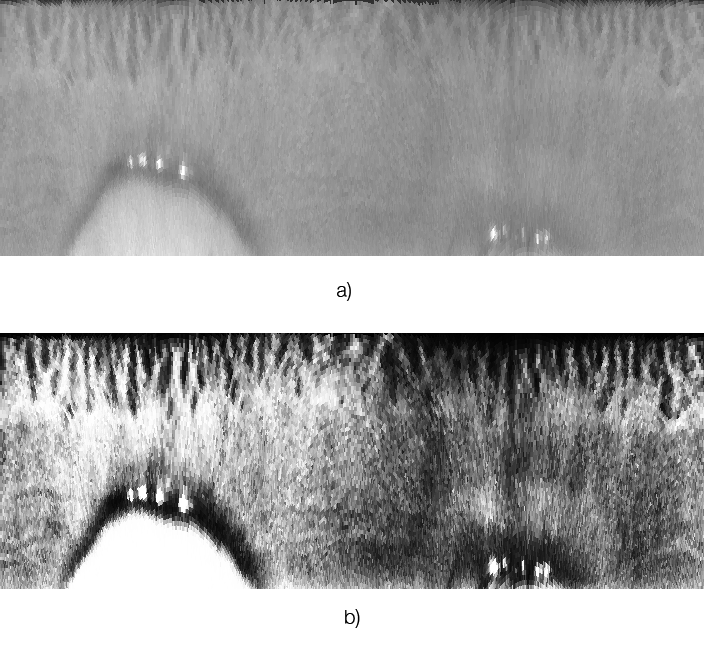
\includegraphics[width=0.99
				\textwidth]{../report/iris/iris_unrolled.png} \caption{a) original cropped iris pattern b) equalized iris pattern - single features are more easily detectable} \label{fig:unrolled_iris} 
			\end{figure}
		\end{column}
	\end{columns}
\end{frame}
\subsection{Pattern Generation} 
\begin{frame}
	[fragile] \frametitle{Gabor and Log-Gabor filtering} 
	\begin{columns}
		\begin{column}
			{0.5
			\textwidth} 
			\begin{figure}
				[t] \centering 
				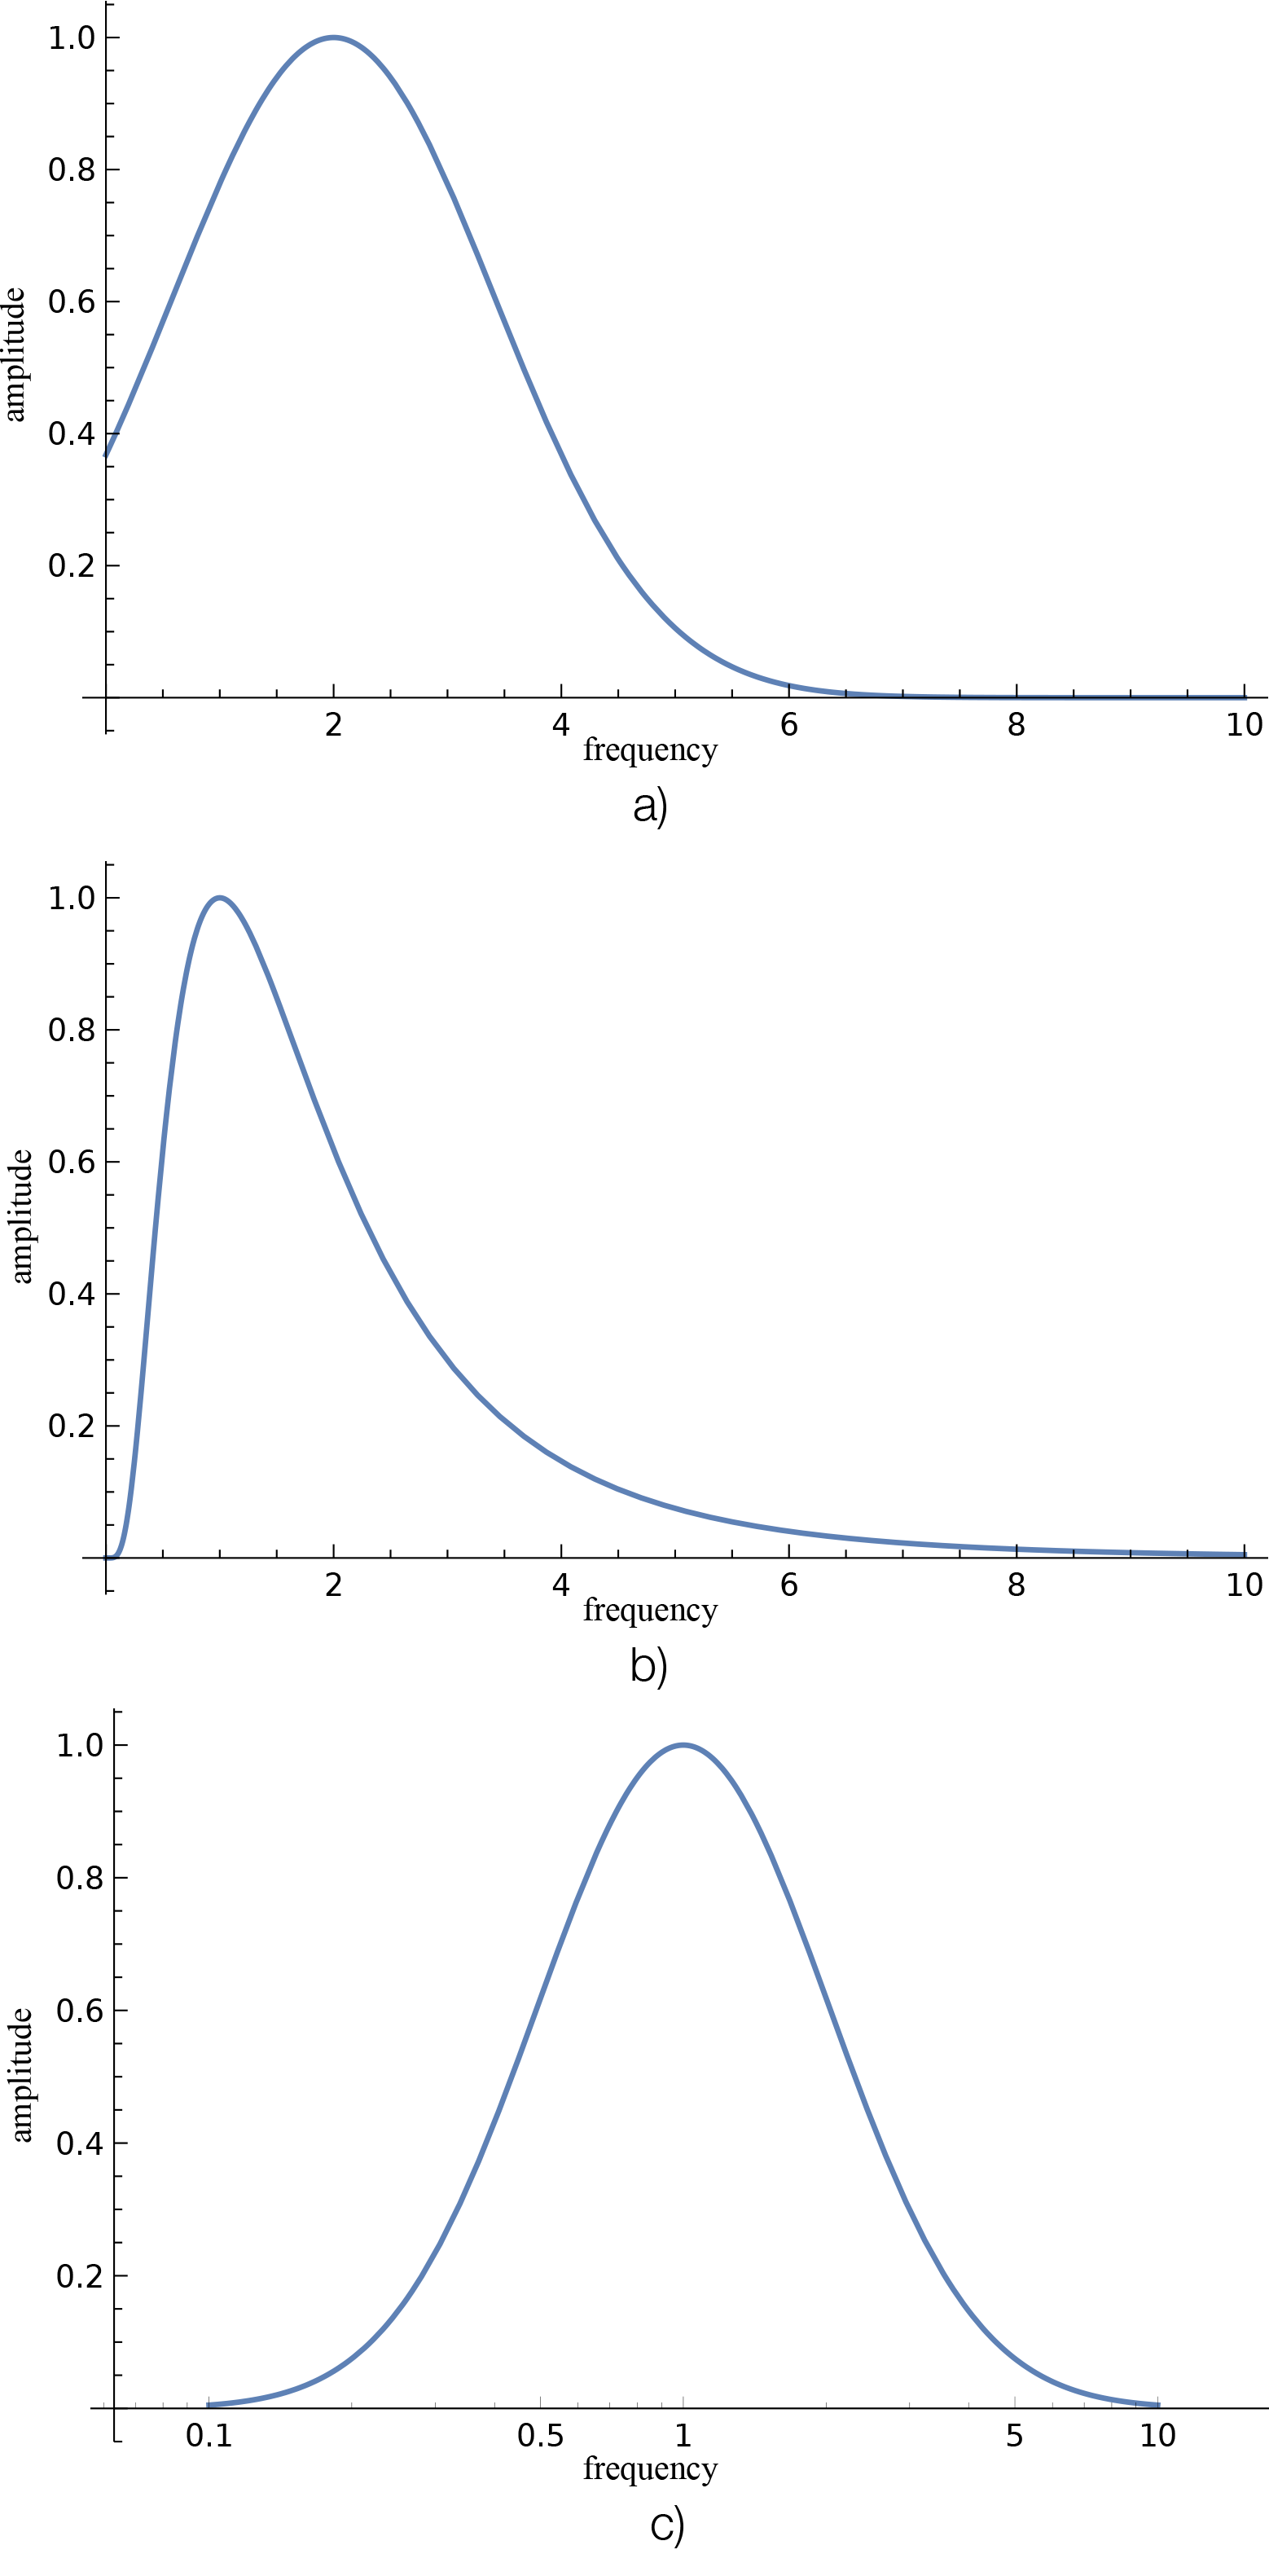
\includegraphics[width=0.62
				\textwidth]{../report/iris/freq_response_gabor.png} \label{fig:frequency_response} 
			\end{figure}
		\end{column}
		\begin{column}
			{0.5
			\textwidth} 
			\begin{figure}
				[t] \centering 
				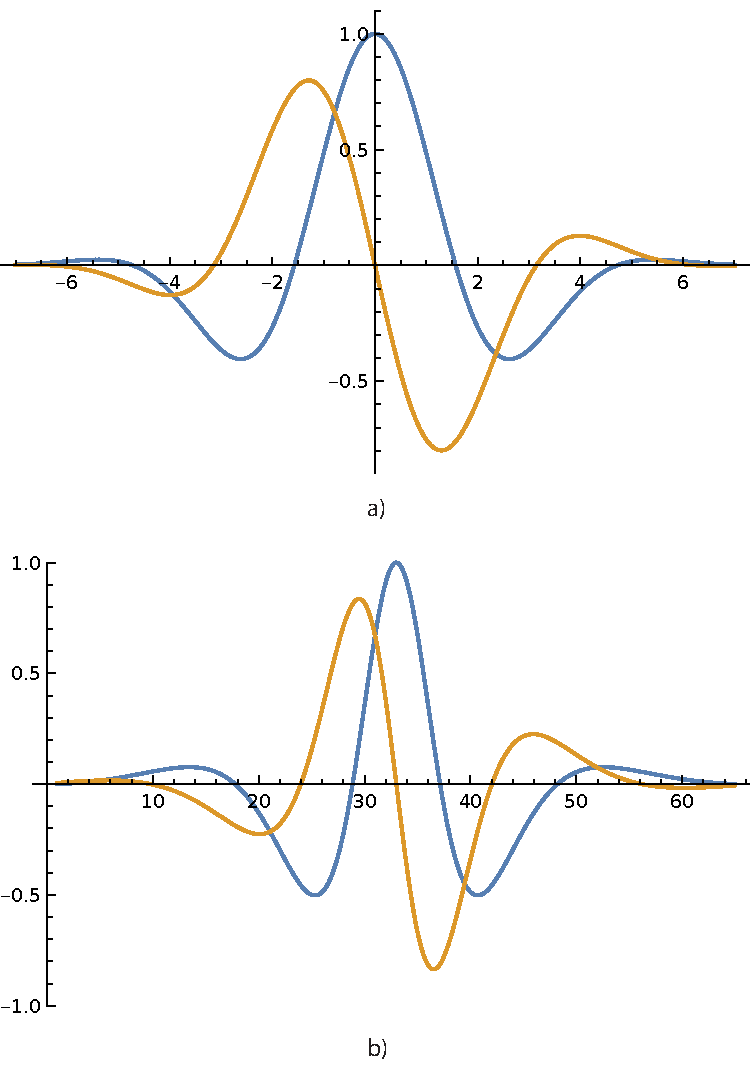
\includegraphics[width=0.89
				\textwidth]{../report/iris/impulse_response} \label{fig:impulse_response} 
			\end{figure}
		\end{column}
	\end{columns}
\end{frame}

\begin{frame}
	[fragile] \frametitle{2D - Log Gabor}
	
	\begin{columns}
		\begin{column}
			{0.5
			\textwidth} 
			\begin{figure}[H]
			\centering
			  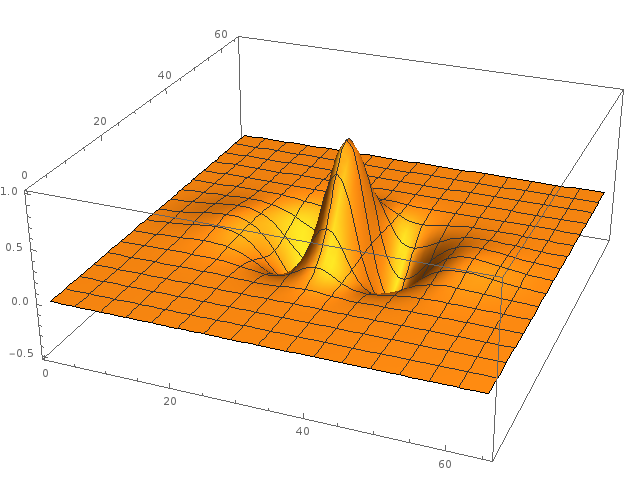
\includegraphics[width=0.89\textwidth]{../report/iris/log_gabor_2d.png}
				\caption{3D representation of a Log Gabor filter's real part in the space domain.}
				\label{fig:2Dloggabor}
			\end{figure}
		\end{column}
		\begin{column}
			{0.5
			\textwidth} 
			\begin{figure}[t]
				\centering
			  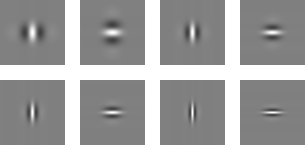
\includegraphics[width=0.49\textwidth]{../report/iris/2d_log_gabor_filter.png}
				\caption{Small subset of the Log Gabor filter bank used, showing different frequencies and orientations}
				\label{fig:filter_bank}
			\end{figure}
		\end{column}
	\end{columns}
	
\end{frame}

\subsection{Pattern Matching} 
\section{Iris} 
\subsection{Iris Database}
\begin{frame}
\frametitle{Iris Database} 
We need a Database to store our iris vectors.\\
What are the requirements for such database?\\
  \begin{itemize}
    \item Fast read cycles
    \item Ability to handle big amounts of data
    \item Efficient API
    \item $[$Optional$]$ CUDA support
  \end{itemize}
%    \begin{figure}[hp]
%       \includegraphics[width=0.40\textwidth]{../figures/ev_network.JPG}
%       \caption{Handle a complex system by using an EOS.}
%     \label{fig:flow}
%   \end{figure} 
\end{frame}

\begin{frame}
\frametitle{Iris Database} 
We use mongoDB(NoSQL) to store our iris vectors.\\
The main reasons for this step were:\\
  \begin{itemize}
    \item NoSQL approach
    \item C/C++/.. API
    \item Master-Slave-Replication
    \item Homebrew CUDA support \footnote{https://github.com/harishd10/mongodb}
  \end{itemize}
  Iris Vector Format: $[$ ID, SUBKEY, IRIS-DATA $]$
\end{frame}


\begin{frame}
\frametitle{Iris Database} 
Main program contains the basic functionalities: \\insert(vector), search(threshold)
    \begin{figure}[hp]
       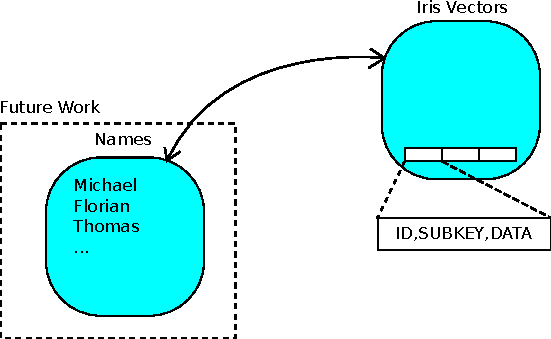
\includegraphics[width=0.60\textwidth]{../report/iris/Database_Approach.pdf}
       \caption{Database handling for the iris storage.}
     \label{fig:flow}
   \end{figure} 
\end{frame}

\begin{frame}
\frametitle{Iris Database} 
Search functionality were implemented by calculating differences.\\
These process is realized by calculating the differences of all vectors in the wholed database to the searched one.\\
\[
dist = \sqrt{\sum_{k=0}^{32}{(vector1[k]-vector2[k])}^2}
\]
By generating $n$ instances, it is possible to divide the matching time by $n$.\\
This is possible since mongoDB use master slave replication.
\end{frame}

\section{Implementation} 
\subsection{Program} 
\begin{frame}
\end{frame}
\begin{frame}
	[allowframebreaks] \frametitle{References} 
	\bibliographystyle{amsalpha} 
	\bibliography{../report/jabrefmaster.bib} 
\end{frame}
\end{document} 
